\documentclass{unswmaths}

\usepackage{unswshortcuts}
\usepackage[all]{xy}
\usepackage{csquotes}

\begin{document}

\subject{Algebraic Topology}
\author{Edward McDonald}
\title{Assignment 1}
\studentno{z3375335}

\newcommand{\Hilb}{\mathcal{H}}
\newcommand{\Proj}{\mathbf{P}}
\newcommand{\M}{\mathcal{M}}
\newcommand{\Dom}{\operatorname{Dom}}
\newcommand{\D}{\delta}
\newcommand{\Di}{\mathcal{D}}
\newcommand{\sgn}{\operatorname{sgn}}
\newcommand{\Ha}{\mathcal{H}}
\newcommand{\Span}{\operatorname{span}}
\newcommand{\im}{\operatorname{im}}

\setlength\parindent{0pt}

\unswtitle{}

\section*{Question 1}
Let $A = \{a,b,c,d\}$ be an ordered set, ordered alphabetically. 
\begin{proposition}
    Let 
    \begin{equation*}
        K = \{a,b,c,d,ab,bc,bd\}
    \end{equation*}
    and
    \begin{equation*}
        K' = \{a,b,c,d,ab,bc,abc\}.
    \end{equation*}
    Then $K$ is a simplicial complex, and $K'$ is not.
\end{proposition}
\begin{proof}
    We need to check that $K$ is closed under taking non-empty
    subsets. Indeed, the only elements of $K$ which are not singletons
    are $ab,bc,bd$, and the only non-empty subsets of these are $a,b,c,d$,
    which are contained in $K$. Hence $K$ is a simplicial complex.
    
    However, we have $abc \in K'$, and $ac \subset abc$ but $ac \notin K'$.
    Hence $K'$ is not a simplicial complex.
\end{proof}

\begin{proposition}
    If 
    \begin{equation*}
        K = \{a,b,c,d,ab,bc,bd\}
    \end{equation*}
    then we can visualise $|K|$ as\\
    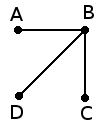
\includegraphics[width=40mm]{polytope.png}
\end{proposition}
\begin{proof}
    There are only four singletons in $K$, so therefore four vertices.
    There are no three element subjects, so the only simplices in $K$
    can be $1$-simplexes. So there are four vertices, and since
    there are three two element subsets, we have three lines. They 
    are the lines joining $a$ to $b$, $b$ to $c$ and $b$ to $d$.
\end{proof}

\section*{Question 2}
\begin{proposition}
    Let $\phi:\Itgr\rightarrow\Itgr\oplus\Itgr$ be given by $\phi(n) = (n,-2n)$
    and $\psi:\Itgr\oplus\Itgr\rightarrow \Itgr$ be $\psi(n,m) = 2n+m$. Then
    \begin{equation*}
        0\xrightarrow{}\Itgr\xrightarrow{\phi}\Itgr\oplus\Itgr\xrightarrow{\psi}\Itgr\xrightarrow{} 0
    \end{equation*}
    is a chain complex. 
    
    The homology groups are all $0$, i.e. the trivial group.
\end{proposition}
\begin{proof}
    We only need to check that $\im\phi \subseteq \ker\psi$. Let $(n,-2n) \in \im\phi$.
    Then $\psi(n,-2n) = 2n-2n = 0$. Hence $(n,-2n) \in \ker\psi$. Thus we
    have a chain complex.
    
    Starting from the left, the first homology group is just $\ker(\phi)$.
    But we have $\phi(n) = 0$ if and only if $(n,-2n) = (0,0)$,
    so this is true if and only if $n = 0$. Thus $\ker\phi = 0$. 
    
    The next homology group is $\ker\psi/\im\phi$.
    
    Let $(n,m) \in \ker\psi$. Then $2n+m = 0$, so $m = -2n$.
    Thus $(n,m) = \phi(n)$. Therefore, $\ker\psi \subseteq \im\phi$.
    Hence $\ker\psi/\im\phi$ is the trivial group.
    
    The final homology group is $\ker(\Itgr\rightarrow 0)/\im\psi$.
    Now $\ker(\Itgr\rightarrow 0) = \Itgr$, however $\im\psi = \Itgr$
    since if $n \in \Itgr$ we can write $n = \psi(0,n)$. Hence
    the final cohomology group is $\Itgr/\im\psi = \Itgr/\Itgr$. So all
    homology groups are trivial.
\end{proof}

\section*{Question 3}
For this question, we let $K$ be the simplicial complex associated
to the following labelled surface diagram,\\
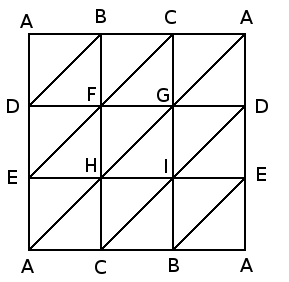
\includegraphics[width=40mm]{klein.png}\\
\begin{proposition}
    The homology of $K$ is as follows,
    \begin{align*}
        H_p(K) &\isom 0\text{ for }p \geq 3\\
        H_2(K) &\isom 0\\
        H_1(K) &\isom  \Itgr/2\Itgr \oplus \Itgr\\
        H_0(K) &\isom \Itgr\\
        H_p(K) &\isom 0\text{ for }p < 0.
    \end{align*}
\end{proposition}
\begin{proof}
There are no $p$-chains in $K$ for $p \geq 3$, so for $p \geq 3$ we have $C_p(K) = 0$. 
Hence $H_p(K) = 0$. Similarly for $p < 0$ we have $C_p(K) = 0$, so $H_p(K) = 0$.

The only potentially non-trivial cases are $p = 0,1,2$.

First we compute $H_0(K)$. Since $C_{-1}(K) = 0$, we have $\ker(\partial_0) = C_0(K)$. 

Now if $x,y \in C_0(K)$, since $|K|$ is connected we can create a path $x_0,x_1,x_2,\ldots,x_n$
such that $x = x_0$ and $y = x_n$ so that $x-y = \partial_1([x_0x_1]+[x_1x_2]+\cdots+[x_{n-1}x_n])$.
Hence $x$ and $y$ are in the same congruence class modulo $B_0(K)$. Thus
there is only one congruence class for all the points of $K$, thus
$H_0(K) \isom \Itgr$.

Let $L$ be the subcomplex
generated by $\{a,b,c,d,e\}$.

Now we compute $H_1(K):= \ker\partial_1/\im\partial_2$. We have,
\begin{equation*}
    [AB]+[BC]+[CA],\;[AD]+[DE]+[EA] \in \ker\partial_1.
\end{equation*}
We wish to show that these are generators for $H_1(K)$. 
To this end, we wish to show that any element of $\ker(\partial_1)$
is homologous to an element carried by $C_1(L)$. 

Let $c \in \ker(\partial_1)$. We need to show that we can add
elements of $B_1(K)$ to $c$ to obtain a chain carried by $L$.

Add multiples of elements of $B_1(K)$ to $c$ corresponding to the simplices
labelled in the following order:\\
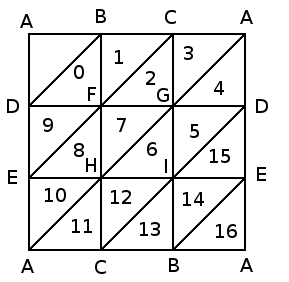
\includegraphics[width=40mm]{klein4.png}\\
So that the only edges which are not annihilated are the ones shown below:\\
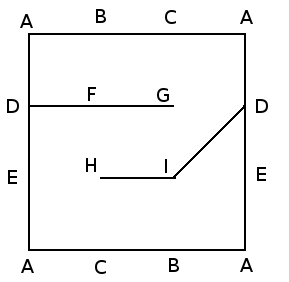
\includegraphics[width=40mm]{klein5.png}\\
Hence $c$ is homologous to a chain carried by the above edges. Now write,
\begin{equation*}
    c+B_1(K) = \sum_{\sigma \in K,|\sigma| = 2} m_\sigma \sigma + B_1(K).
\end{equation*}
where the only coefficients $m_\sigma$ not equal to zero are the ones shown above.
Now since $\partial_1(c) = 0$, we must have that $n_{FG} = n_{DF} = 0$,
and $n_{HI} = n_{DI} = 0$. 

Hence $c$ is homologous to a chain carried by $L$. 

Let $b \in \ker(\partial_1)\cap C_1(L) = Z_1(L)$. Suppose
that
\begin{equation*}
    b = \sum_{\sigma \in L,|\sigma| = 2} k_\sigma \sigma.
\end{equation*}
Then we must have $k_{AB} = k_{BC} = k_{AC}$, 
since if $\partial_2(B) = 0$, we 
need $k_{AB}-k_{BC} = k_{AC}-k_{BC} = 0$. 
Similarly, we must have $k_{AD} = k_{DE} = k_{AE}$.

Hence, $b$ is in the subspace generated
by
\begin{equation*}
    [AB]+[BC]+[CA],\;[AD]+[DE]+[EA] \in \ker\partial_1.
\end{equation*}
Hence $H_1(K)$ is the subgroup generated
by these two elements. Since the first one
has order $2$ and the second has order $0$, this means
\begin{equation*}
    H_1(K) \isom \Itgr\times \Itgr/2\Itgr.
\end{equation*}

To compute $H_2(K)$, note that $C_3(K) = 0$, since there are no $3$-simplices
in $K$. Hence $H_2(K) = \ker\partial_2$. Suppose that $c \in C_2(K)$ is a chain
such that $\partial_2(C)$ is carried by $L$. Let
\begin{equation*}
    c = \sum_{\sigma \in K,|\sigma| = 3} n_\sigma \sigma.
\end{equation*}
Now we prove that all the $n_\sigma$ are equal.

Let $\sigma_0 = K_{FGH}$. Then none of the lines composing the boundary of $\sigma_0$
are in $L$, so if we consider all the simplicies surrounding $\sigma_0$, which we call
$\sigma_1$,$\sigma_2$,$\sigma_3$. If we label the simplex $\sigma_i$
with the number $i$, this is\\
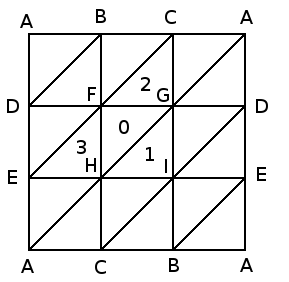
\includegraphics[width=40mm]{klein2.png}\\
We see that we must have $n_{\sigma_0} = n_{\sigma_1} = n_{\sigma_2} = n_{\sigma_3}$,
since the edges $FG$, $FH$ and $HG$ are not in $L$.
We now expand outward, labelling the simplices $\sigma_i$, for $i > 3$, as follows,\\
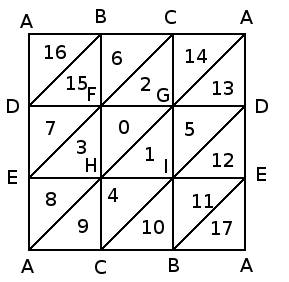
\includegraphics[width=40mm]{klein3.png}\\
See that since the interior edges must cancel out, we must have 
that all the $n_\sigma$ are equal. Hence,
\begin{equation*}
    c = n\sum_{\sigma \in K,|\sigma| =3} \sigma
\end{equation*}
For some $n \in \Itgr$.

Now we compute $\partial_2(c)$. 
\begin{equation*}
    \partial_2(c) = n\sum_{\sigma \in K,|\sigma| = 3} \partial_2(\sigma) = 2nK_{DE}.
\end{equation*}
Hence $\partial_2(c) = 0$ if and only if $n = 0$, so $c = 0$. Hence $\ker(\partial_2) = 0$,
so $H_2(K) = 0$.


\end{proof}

\section*{Question 4}
\begin{proposition}
    Suppose that $f_{1\bullet},f_{2\bullet}:C_\bullet\rightarrow C_\bullet'$
    be chain maps, and suppose $s_\bullet$ is a chain homotopy from $f_{1\bullet}$
    to $f_{2\bullet}$. 
    
    Suppose $g_{\bullet}:C_\bullet'\rightarrow C_\bullet''$ is another chain map.
    
    Then there is a homotopy from $g_\bullet f_{1\bullet}$ to $g_\bullet f_{1\bullet}$.
\end{proposition}
\begin{proof}
    Let $p \in \Itgr$. Then we have,
    \begin{equation*}
        f_{1p}-f_{2p} = \partial'_{p+1}s_p+s_{p-1}\partial_p.
    \end{equation*}
    Hence, since $g_p$ is a homomorphism of abelian groups,
    \begin{equation*}
        g_pf_{1p}-g_pf_{2p} = g_p\partial'_{p+1}s_p+g_{p}s_{p-1}\partial_p.
    \end{equation*}
    However by assumption, $g_\bullet$ is a chain map. So $g_p \partial'_{p+1} = \partial''_{p+1} g_{p+1}$.
    
    Define $t_p := g_{p}s_{p-1}$. Then we have
    \begin{equation*}
        g_pf_{1p} - g_pf_{2p} = \partial''_{p+1}t_{p+1}+t_p\partial_p.
    \end{equation*}
    Hence $t_\bullet$ is a homotopy from $g_\bullet f_{1\bullet}$ to $g_\bullet f_{2\bullet}$.
\end{proof}

\section*{Question 5}

The following is a useful lemma from general topology. I am including
it here since I cannot find a good reference for it.
\begin{lemma}
\label{topIsom}
    Let $X$ and $Y$ be compact Hausdorff spaces. Suppose that $\varphi:X\rightarrow Y$
    is continuous. The quotient space $X/\varphi$ is the space
    of equivalence classes where $x$ is equivalent to $y$ when $\varphi(x) = \varphi(y)$
    given the quotient topology. The image space $\im \varphi$ is given the subspace
    topology from $Y$. Then we have a homeomorphism,
    \begin{equation*}
        X/\varphi \isom \im\varphi.
    \end{equation*}
\end{lemma}
\begin{proof}
    Define $\psi:X/\varphi\rightarrow \im\varphi$ as follows. 
    
    Let $[x] \in X/\varphi$ be the equivalence class containing $x$. Define
    $\psi([x]) = \varphi(x)$. This is well defined, since if $\varphi(x) = \varphi(y)$,
    then $\psi([x]) = \psi([y])$.
    
    $\psi$ is surjective since if $\varphi(x) \in \im\varphi$, then $\varphi(x) = \psi([x])$. 
    
    Let $\pi:X\rightarrow X/\varphi$ denote the quotient map.
    
    Now we must show that $\psi$ is continuous. Let $U \subseteq \im\varphi$ be open.
    Then $U = \im\varphi \cap V$ for some open $V \subseteq \varphi$. Then $\varphi^{-1}(V)$
    is open in $X$. Hence, since $\varphi = \psi \circ \pi$, we have that
    $\varphi^{-1}(V) = \pi^{-1}\circ\psi^{-1}(V)$. Since $X/\varphi$
    is given the topology, we have $W \subseteq X/\varphi$ is open if and only
    if $\pi^{-1}(W)$ is open in $X$. Hence, $\psi^{-1}(V) = \psi^{-1}(U)$
    is open in $X/\varphi$.
    
    Hence $\psi$ is continuous. We also have that $\psi$ is injective,
    since if $\psi([x]) = \psi([y])$, then $\varphi(x) = \varphi(y)$, so $[x] = [y]$.
    
    Let $K \subseteq X/\varphi$ be closed. Hence it is compact, hence $\psi(K)$
    is compact, hence closed since $Y$ is Hausdorff. 
    
    Thus $\psi$ is a closed continuous bijection, hence a homeomorphism.
\end{proof}

\begin{proposition}
    Let $K$ be a simplicial complex, and let $X$ be a topological
    space such that $\theta:|K|\rightarrow X$ is a triangulation. 
    Define
    \begin{equation*}
        Y := (X \times [0,1])/\sim
    \end{equation*}
    where $\sim$ is the equivalence relation generated by $(x,1) \sim (x',1)$
    for all $x,x' \in X$. Denote the equivalence class containing the point $(x,t)$
    by $[(x,t)]_\sim$.
    Then a triangulation for $Y$ is given by the simplicial complex, $K' = K*w$,
    where $w \notin K^{(0)}$ is a new vertex, and $K*w$ denotes the cone
    on $K$.
\end{proposition}
\begin{proof}
    Let $T:X\rightarrow |K|$ be the inverse of the triangulation, $T = \theta^{-1}$,
    and let $n$ be the number of vertices of $K$. 
    
    Let $T':X\times [0,1]\rightarrow |K|\times [0,1]$ be the product map 
    such that $T'(x,t) = (T(x),t)$ for all $x \in X$ and $t \in [0,1]$.
    
    Now we define a continuous surjection $\varphi: |K| \times [0,1] \rightarrow |K'|$.
    
    Let $\iota:|K|\rightarrow |K'|$ be the embedding, so that $\iota(p) = (p,0)$
    for $p \in |K|$. Now if $t \in [0,1]$ and $p \in |K|$, define $\varphi(p,t) = (p(1-t),t)$.
    
    Hence $\varphi(p,t) \in |K'|$, and $\varphi(p,t) = \varphi(q,s)$ if and only
    if $s = t = 1$. Hence, $\varphi\circ T'$ is a continuous function
    from $X\times [0,1]$ to $|K'|$. Thus by lemma \ref{topIsom}, we have a homeomorphism
    \begin{equation*}
        (X\times [0,1]/\sim)\; \isom |K'|
    \end{equation*}
    where $(x,t) \sim (x',t')$ if and only if $t = t' = 1$.
    
\end{proof}

\end{document}complex
